\documentclass[10pt]{article}
\usepackage[margin=0.8in]{geometry}

\usepackage[utf8]{inputenc}
\usepackage[T1]{fontenc}
\usepackage{amsmath}
\usepackage{amsfonts}
\usepackage{amssymb}
\usepackage[version=4]{mhchem}
\usepackage{stmaryrd}
\usepackage{graphicx}
\usepackage[export]{adjustbox}
\usepackage{bbold}
\usepackage{fixltx2e}
\usepackage{caption}
\usepackage{mathtools}
\usepackage{amsfonts} %% <- also included by amssymb
\DeclareMathSymbol{-}{\mathbin}{AMSa}{"39}
\usepackage[parfill]{parskip}
\usepackage{float}
	
\usepackage[framemethod=TikZ]{mdframed}
\colorlet{shadecolor}{orange!15}
\usepackage{xcolor}
\usepackage{amsthm}
\usepackage{framed}





\begin{document}

\title{Lecture 9:  Analytic Inverse Kinematics (IK)}
\date{Sep. 14, 2023 }
\author{Wanxin Jin}
\maketitle



The inverse kinematics (IK) problem is to determine the joint variables given end-effector position and orientation. The solution to IK is of fundamental importance in order to transform the motion assignment in the end-effector in the operational space into the  joint space motions for control purpose.
The IK problem is  complex since:

\begin{itemize}
  \item Forward kinematics  in general are nonlinear, and thus IK is not always possible to find a closed-form solution.

  \item Multiple or infinite solutions may exist for a IK problem, e.g., in the case of a  redundant manipulator.

  \item There might be no admissible solutions, in view of the manipulator kinematic limits.

\end{itemize}

In this lecture, we only talk about the IK problem that permits a closed-form solution. This is only valid for some special-structured kinematic structures. Those IK solutions are all derived based on geometric intuition. For more generalized case of IK, we will leave it after we have learned differential kinematics.

\section{IK of Three-link Planar Arm}



\begin{figure}[H]
    \centering
   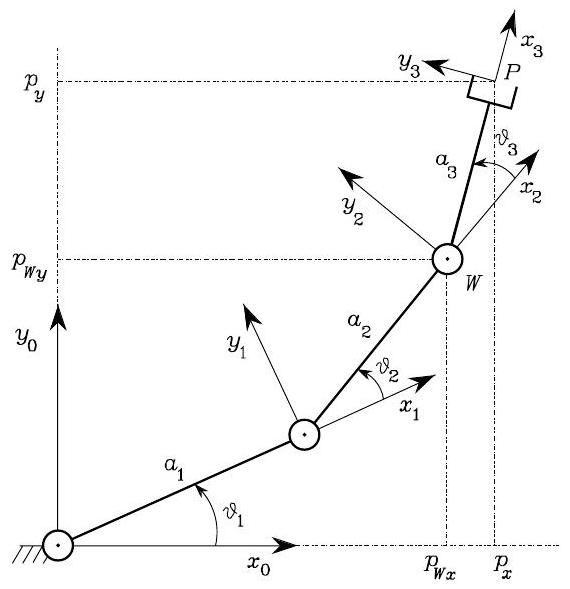
\includegraphics[max width=0.40\textwidth]{./kinematics/3link_arm}
    \label{c1.l2.three-link-robot-arm}
\end{figure}





\noindent
Suppose the pose of the end-effector is specified with its planar position  $(p_{x}, p_{y})$ and the angle $\phi$ with the axis $x_{0}$.  We  want to use IK to find the corresponding joint variables $\boldsymbol{q}=[\vartheta_{1}, \vartheta_{2}, \vartheta_{3}]$.


To achieve so, we first identify the following relation holds

\begin{equation}\label{c1.l2.3link.sum}
    \phi=\vartheta_{1}+\vartheta_{2}+\vartheta_{3}
\end{equation}

\noindent
Also, the following equations can be obtained:

$$
\begin{aligned}
& p_{W x}=p_{x}-a_{3} c_{\phi}=a_{1} c_{1}+a_{2} c_{12} \\
& p_{W y}=p_{y}-a_{3} s_{\phi}=a_{1} s_{1}+a_{2} s_{12}
\end{aligned}
$$

\noindent
which describe the position of point $W$, i.e., the origin of Frame 2;  depending only on   $\vartheta_{1}$ and $\vartheta_{2}$.








The cosine theorem to the triangle formed by links $a_{1}, a_{2}$ and the segment connecting  $W$ and $O$ gives

$$
p_{W x}^{2}+p_{W y}^{2}=a_{1}^{2}+a_{2}^{2}-2 a_{1} a_{2} \cos \left(\pi-\vartheta_{2}\right) ;
$$

Solving $c_2$ leads to

$$
c_{2}=\frac{p_{W x}^{2}+p_{W y}^{2}-a_{1}^{2}-a_{2}^{2}}{2 a_{1} a_{2}}
$$



For the existence of the triangle, it must be $\sqrt{p_{W x}^{2}+p_{W y}^{2}} \leq a_{1}+a_{2}$. This condition is not satisfied when the given point is outside the arm reachable workspace. Then, under the assumption of admissible solutions, it is

$$
\vartheta_{2}= \pm \cos ^{-1}\left(c_{2}\right)
$$


Thus, two admissible $\vartheta_{2}$ are obtained: the elbow-up posture is obtained for $\vartheta_{2} \in(-\pi, 0)$ while the elbow-down posture is obtained for $\vartheta_{2} \in(0, \pi)$, as shown in the figure blow.


\begin{figure}[H]
    \centering
    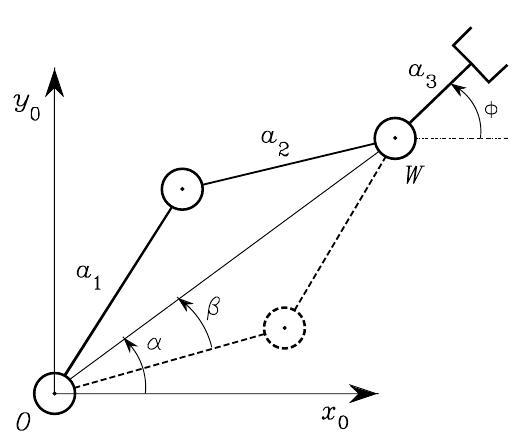
\includegraphics[max width=0.35\textwidth]{./kinematics/postures_2link_arm}
    \caption{Admissible postures for a two-link planar arm}
    \label{fig:enter-label}
\end{figure}




\noindent



\noindent
To find $\vartheta_{1}$ consider the angles $\alpha$ and $\beta$ in the above figure. Notice that the determination of $\alpha$ depends on the sign of $p_{W x}$ and $p_{W y}$; then, it is necessary to compute $\alpha$ as

$$
\alpha=\operatorname{Atan} 2\left(p_{W y}, p_{W x}\right) .
$$

\noindent
To compute $\beta$, applying again the cosine theorem yields

$$
c_{\beta} \sqrt{p_{W x}^{2}+p_{W y}^{2}}=a_{1}+a_{2} c_{2}
$$

\noindent
and resorting to the expression of $c_{2}$ given above leads to

$$
\beta=\cos ^{-1}\left(\frac{p_{W x}^{2}+p_{W y}^{2}+a_{1}^{2}-a_{2}^{2}}{2 a_{1} \sqrt{p_{W x}^{2}+p_{W y}^{2}}}\right)
$$

\noindent
with $\beta \in(0, \pi)$ so as to preserve the existence of triangles. Then, it is

$$
\vartheta_{1}=\alpha \pm \beta
$$

\noindent
where the positive sign holds for $\vartheta_{2}<0$ and the negative sign for $\vartheta_{2}>0$. Finally, $\vartheta_{3}$ is computed from (\ref{c1.l2.3link.sum}).





\section{IK of Manipulators with Spherical Wrist}
Most of manipulators are kinematically simple, since they are typically formed by an arm and a spherical wrist. This choice is partly motivated by the difficulty to find IK in the general case. In particular, a six-DOF kinematic structure has closed-form IK solutions if:

\begin{itemize}
  \item three consecutive revolute joint axes intersect at a common point, like for the spherical wrist;
  \item three consecutive revolute joint axes are parallel, like the three-link robot arm
\end{itemize}

\noindent
Inspired by  IK to a three-link planar arm, an itermediate point on the  manipulator  can be found, such that the IK problem can be decoupled into two lower-dimentional sub-problems. 
Specifically, for a manipulator with spherical wrist, the natural choice is to locate such point $W$ at the wrist position, i.e., at the intersection of the three  revolute axes of the wrist. If the end-effector pose is $\boldsymbol{p}_{e}$ and $\boldsymbol{R}_{e}=\left[\begin{array}{lll}\boldsymbol{n}_{e} & \boldsymbol{s}_{e} & \boldsymbol{a}_{e}\end{array}\right]$, the wrist position will be

$$
\boldsymbol{p}_{W}=\boldsymbol{p}_{e}-d_{6} \boldsymbol{a}_{e}
$$

\begin{figure}[H]
    \centering
    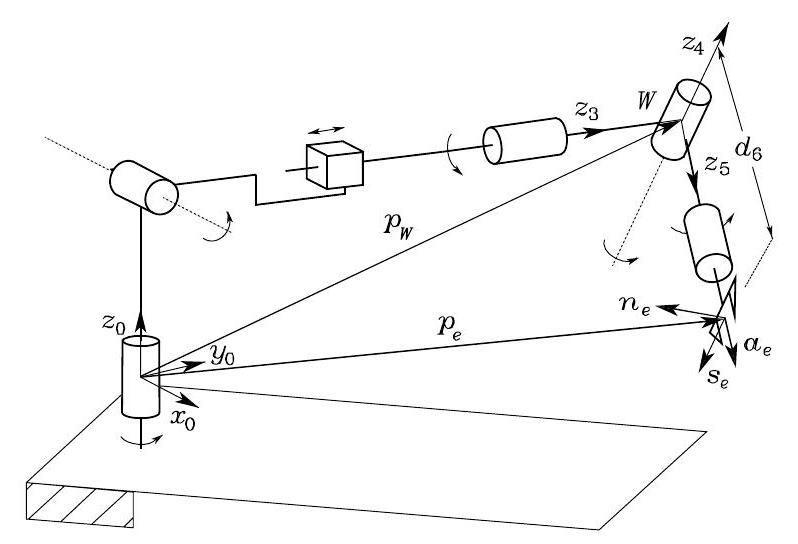
\includegraphics[max width=0.5\textwidth]{./kinematics/analytic_ik_decouple}
    \caption{Manipulator with spherical wrist}
    \label{fig:enter-label}
\end{figure}


\noindent
which is a function of the sole joint variables that determine the arm position. Hence, in the case of a (nonredundant) three-DOF arm, the inverse kinematics can be solved according to the following steps:

\begin{itemize}
  \item Compute the wrist position $\boldsymbol{p}_{W}\left(q_{1}, q_{2}, q_{3}\right)$.

  \item Solve inverse kinematics for $\left(q_{1}, q_{2}, q_{3}\right)$.

  \item Compute $\boldsymbol{R}_{3}^{0}\left(q_{1}, q_{2}, q_{3}\right)$.

  \item Compute $\boldsymbol{R}_{6}^{3}\left(\vartheta_{4}, \vartheta_{5}, \vartheta_{6}\right)=\boldsymbol{R}_{3}^{0 T} \boldsymbol{R}$

  \item Solve inverse kinematics for orientation $\left(\vartheta_{4}, \vartheta_{5}, \vartheta_{6}\right)$

\end{itemize}

Therefore, on the basis of this kinematic decoupling, IK for the arm separately from the IK for the spherical wrist. Below are presented the solutions for two typical arms (spherical and anthropomorphic) as well as the solution for the spherical wrist.

\subsection{IK of Spherical Arm}
Consider the spherical arm:

\begin{figure}[h]
    \centering
   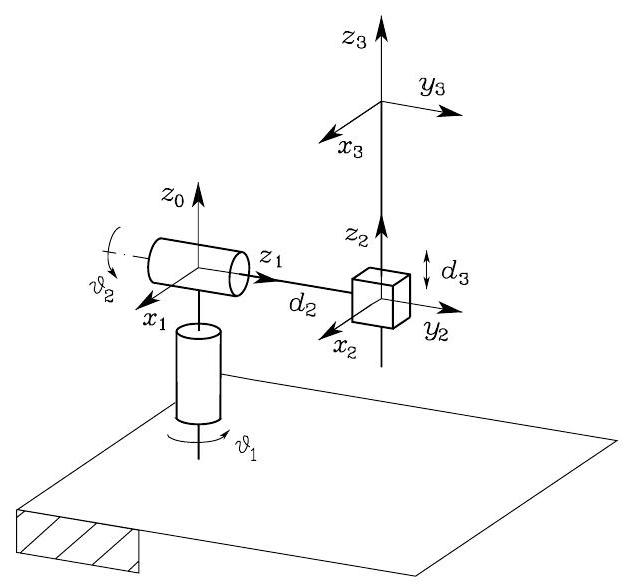
\includegraphics[max width=0.4\textwidth]{./kinematics/spherical_arm}
    \caption{Spherical arm}
    \label{c1.l2.fig.spherical-arm}
\end{figure}

\noindent
Its  kinematics is
$$
\boldsymbol{T}_{3}^{0}(\boldsymbol{q})=\boldsymbol{A}_{1}^{0} \boldsymbol{A}_{2}^{1} \boldsymbol{A}_{3}^{2}=\left[\begin{array}{cccc}
c_{1} c_{2} & -s_{1} & c_{1} s_{2} & c_{1} s_{2} d_{3}-s_{1} d_{2} \\
s_{1} c_{2} & c_{1} & s_{1} s_{2} & s_{1} s_{2} d_{3}+c_{1} d_{2} \\
-s_{2} & 0 & c_{2} & c_{2} d_{3} \\
0 & 0 & 0 & 1
\end{array}\right]
$$


To find the joint variables $\vartheta_{1}, \vartheta_{2}, d_{3}$ corresponding to  $\boldsymbol{p}_{W}=[p_{Wx}, p_{Wy}, p_{Wz}]^T$, we equate the first three elements of the fourth columns of the matrices and thus obtain the following after some equation manipulation

$$
\left[\begin{array}{c}
p_{W x} c_{1}+p_{W y} s_{1} \\
-p_{W z} \\
-p_{W x} s_{1}+p_{W y} c_{1}
\end{array}\right]=\left[\begin{array}{c}
d_{3} s_{2} \\
-d_{3} c_{2} \\
d_{2}
\end{array}\right]
$$

\noindent
Then, solving the above equation for $\vartheta_{1}, \vartheta_{2}, d_{3}$ yields 

$$
\vartheta_{1}=2 \operatorname{Atan} 2\left(-p_{W x} \pm \sqrt{p_{W x}^{2}+p_{W y}^{2}-d_{2}^{2}}, d_{2}+p_{W y}\right)
$$


$$
\vartheta_{2}=\operatorname{Atan} 2\left(p_{W x} c_{1}+p_{W y} s_{1}, p_{W z}\right)
$$

$$
d_{3}=\sqrt{\left(p_{W x} c_{1}+p_{W y} s_{1}\right)^{2}+p_{W z}^{2}}
$$


\subsection{IK of Anthropomorphic Arm}


Consider the anthropomorphic arm:

\begin{figure}[H]
    \centering
   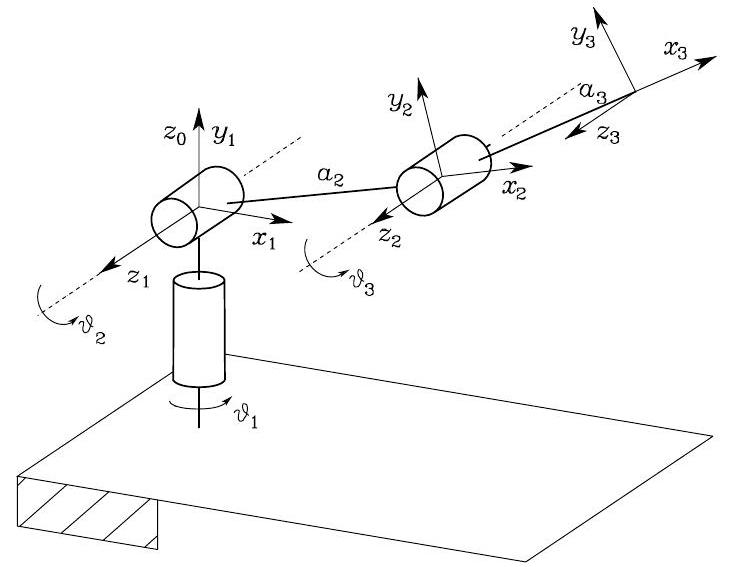
\includegraphics[max width=0.3\textwidth]{./kinematics/anthropomorphic_arm}
   \caption{Anthropomorphic arm}
\end{figure}




$$
\boldsymbol{T}_{3}^{0}(\boldsymbol{q})=\boldsymbol{A}_{1}^{0} \boldsymbol{A}_{2}^{1} \boldsymbol{A}_{3}^{2}=\left[\begin{array}{cccc}
c_{1} c_{23} & -c_{1} s_{23} & s_{1} & c_{1}\left(a_{2} c_{2}+a_{3} c_{23}\right) \\
s_{1} c_{23} & -s_{1} s_{23} & -c_{1} & s_{1}\left(a_{2} c_{2}+a_{3} c_{23}\right) \\
s_{23} & c_{23} & 0 & a_{2} s_{2}+a_{3} s_{23} \\
0 & 0 & 0 & 1
\end{array}\right]
$$



To find the joint variables $\vartheta_{1}, \vartheta_{2}, d_{3}$ corresponding to  $\boldsymbol{p}_{W}=[p_{Wx}, p_{Wy}, p_{Wz}]^T$, we equate the first three elements of the fourth columns of the matrices and thus obtain the following 


$$
\begin{aligned}
& p_{W x}=c_{1}\left(a_{2} c_{2}+a_{3} c_{23}\right) \\
& p_{W y}=s_{1}\left(a_{2} c_{2}+a_{3} c_{23}\right) \\
& p_{W z}=a_{2} s_{2}+a_{3} s_{23} .
\end{aligned}
$$


\noindent
There exist four solutions:

$$
\left(\vartheta_{1, \mathrm{I}}, \vartheta_{2, \mathrm{I}}, \vartheta_{3, \mathrm{I}}\right) \quad\left(\vartheta_{1, \mathrm{I}}, \vartheta_{2, \mathrm{III}}, \vartheta_{3, \mathrm{II}}\right) \quad\left(\vartheta_{1, \mathrm{II}}, \vartheta_{2, \mathrm{II}}, \vartheta_{3, \mathrm{I}}\right) \quad\left(\vartheta_{1, \mathrm{II}}, \vartheta_{2, \mathrm{IV}}, \vartheta_{3, \mathrm{II}}\right)
$$

with 

$$
c_{3}=\frac{p_{W x}^{2}+p_{W y}^{2}+p_{W z}^{2}-a_{2}^{2}-a_{3}^{2}}{2 a_{2} a_{3}}
$$



$$
s_{3}^+= \sqrt{1-c_{3}^{2}}\quad\quad s_{3}^-= -\sqrt{1-c_{3}^{2}}
$$



$$
\begin{aligned}
\vartheta_{3, \mathbf{I}}&=\operatorname{Atan} 2 \left( s_3^{+}, c_{3}\right)\\
\vartheta_{3, \mathrm{II}} & =\operatorname{Atan} 2 \left( s_3^{-}, c_{3}\right)
\end{aligned}
$$



$$
\begin{aligned}
\vartheta_{1, \mathrm{I}} & =\operatorname{Atan} 2\left(p_{W y}, p_{W x}\right) \\
\vartheta_{1, \mathrm{II}} & =\operatorname{Atan} 2\left(-p_{W y},-p_{W x}\right) .
\end{aligned}
$$


$$
\begin{aligned}
\vartheta_{2, \mathrm{I}}=\operatorname{Atan} 2 & \left(\left(a_{2}+a_{3} c_{3}\right) p_{W z}-a_{3} s_{3}^{+} \sqrt{p_{W x}^{2}+p_{W y}^{2}},\right. 
\left.\left(a_{2}+a_{3} c_{3}\right) \sqrt{p_{W x}^{2}+p_{W y}^{2}}+a_{3} s_{3}^{+} p_{W z}\right) \\
\vartheta_{2, \mathrm{II}}=\operatorname{Atan} 2 & \left(a_{2}+a_{3} c_{3}\right) p_{W z}+a_{3} s_{3}^{+} \sqrt{p_{W x}^{2}+p_{W y}^{2}},  \left.-\left(a_{2}+a_{3} c_{3}\right) \sqrt{p_{W x}^{2}+p_{W y}^{2}}+a_{3} s_{3}^{+} p_{W z}\right)
\end{aligned}
$$


$$
\begin{aligned}
\vartheta_{2, \mathrm{III}}=\operatorname{Atan2} & \left(\left(a_{2}+a_{3} c_{3}\right) p_{W z}-a_{3} s_{3}^{-} \sqrt{p_{W x}^{2}+p_{W y}^{2}},\right.  \left.\left(a_{2}+a_{3} c_{3}\right) \sqrt{p_{W x}^{2}+p_{W y}^{2}}+a_{3} s_{3}^{-} p_{W z}\right) \\
\vartheta_{2, \mathrm{IV}}=\operatorname{Atan} 2 & \left(\left(a_{2}+a_{3} c_{3}\right) p_{W z}+a_{3} s_{3}^{-} \sqrt{p_{W x}^{2}+p_{W y}^{2}},\right.  \left.-\left(a_{2}+a_{3} c_{3}\right) \sqrt{p_{W x}^{2}+p_{W y}^{2}}+a_{3} s_{3}^{-} p_{W z}\right)
\end{aligned}
$$






\noindent
which are illustrated below: shoulder-right/elbow-up, shoulder-left/elbowup, shoulder-right/elbow-down, shoulder-left/elbow-down; obviously, the forearm orientation is different for the two pairs of solutions. 


\begin{figure}[H]
    \centering
    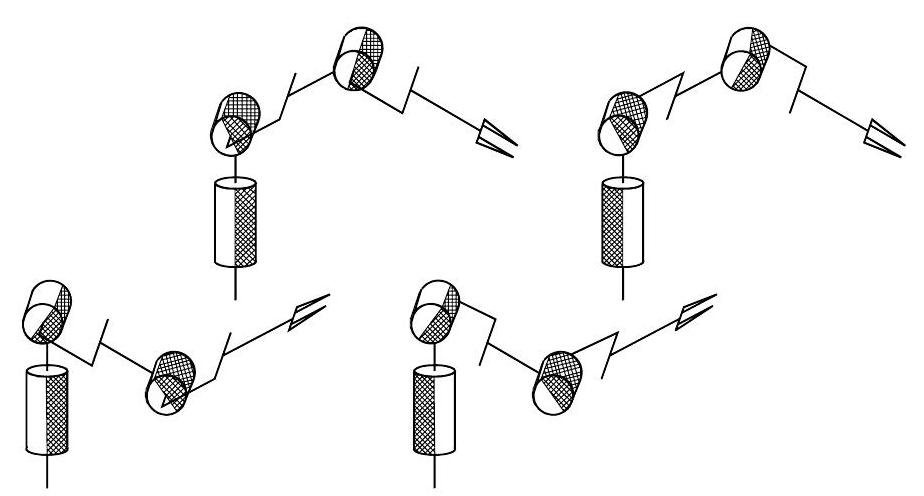
\includegraphics[max width=0.55\textwidth]{./kinematics/4IK_solutions_anthropomorphic_arm}
    \caption{The four configurations of an anthropomorphic arm compatible with a given wrist position}
    \label{fig:enter-label}
\end{figure}


\subsection{IK of Spherical Wrist}
Consider the spherical wrist below.

\begin{figure}[H]
    \centering
   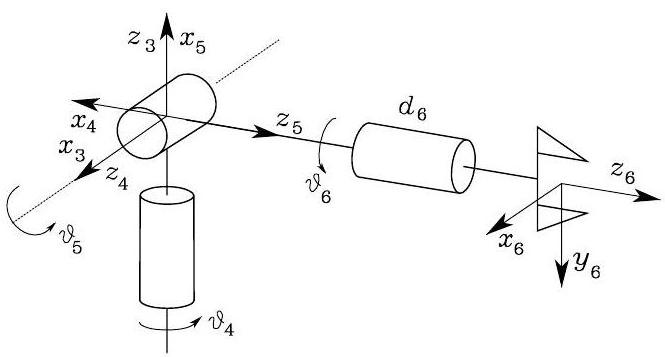
\includegraphics[max width=0.45\textwidth]{./kinematics/spherical_wrist}
    \caption{Spherical wrist}
    \label{c1.l2.fig.spherical-wrist}
\end{figure}

\noindent
To find the joint variables $\vartheta_{4}, \vartheta_{5}, \vartheta_{6}$ corresponding to a given end-effector orientation $\boldsymbol{R}_{6}^{3}$. As previously pointed out, these angles constitute a set of Euler angles ZYZ with respect to Frame 3.


$$
\boldsymbol{R}_{6}^{3}=\left[\begin{array}{rrr}
n_{x}^{3} & s_{x}^{3} & a_{x}^{3} \\
n_{y}^{3} & s_{y}^{3} & a_{y}^{3} \\
n_{z}^{3} & s_{z}^{3} & a_{z}^{3}
\end{array}\right]
$$

\noindent
from its expression in terms of the joint variables, it is possible to compute

$$
\begin{aligned}
& \vartheta_{4}=\operatorname{Atan} 2\left(a_{y}^{3}, a_{x}^{3}\right) \\
& \vartheta_{5}=\operatorname{Atan} 2\left(\sqrt{\left(a_{x}^{3}\right)^{2}+\left(a_{y}^{3}\right)^{2}}, a_{z}^{3}\right) \\
& \vartheta_{6}=\operatorname{Atan} 2\left(s_{z}^{3},-n_{z}^{3}\right)
\end{aligned}
$$

\noindent
for $\vartheta_{5} \in(0, \pi)$, and

$$
\begin{aligned}
& \vartheta_{4}=\operatorname{Atan} 2\left(-a_{y}^{3},-a_{x}^{3}\right) \\
& \vartheta_{5}=\operatorname{Atan} 2\left(-\sqrt{\left(a_{x}^{3}\right)^{2}+\left(a_{y}^{3}\right)^{2}}, a_{z}^{3}\right) \\
& \vartheta_{6}=\operatorname{Atan} 2\left(-s_{z}^{3}, n_{z}^{3}\right)
\end{aligned}
$$

\noindent
for $\vartheta_{5} \in(-\pi, 0)$



\end{document}





% \subsubsection{Closed Chain}
% The above direct kinematics method based on the DH convention exploits the inherently recursive feature of an open-chain manipulator. Nevertheless, the method can be extended to the case of manipulators containing closed kinematic chains according to the technique illustrated below.

% Consider a closed-chain manipulator constituted by $n+1$ links. Because of the presence of a loop, the number of joints $l$ must be greater than $n$; in particular, it can be understood that the number of closed loops is equal to $l-n$.

% With reference to Fig. 2.17, Links 0 through $i$ are connected successively through the first $i$ joints as in an open kinematic chain. Then, Joint $i+1^{\prime}$ connects Link $i$ with Link $i+1^{\prime}$ while Joint $i+1^{\prime \prime}$ connects Link $i$ with Link $i+1^{\prime \prime}$; the axes of Joints $i+1^{\prime}$ and $i+1^{\prime \prime}$ are assumed to be aligned. Although not represented in the figure, Links $i+1^{\prime}$ and $i+1^{\prime \prime}$ are members of the closed kinematic chain. In particular, Link $i+1^{\prime}$ is further connected to Link $i+2^{\prime}$ via Joint $i+2^{\prime}$ and so forth, until Link $j$ via Joint $j$. Likewise, Link $i+1^{\prime \prime}$ is further connected to Link $i+2^{\prime \prime}$ via Joint $i+2^{\prime \prime}$ and so forth, until Link $k$ via Joint $k$. Finally, Links $j$ and $k$ are connected together at Joint $j+1$ to form a closed chain. In general, $j \neq k$.

% In order to attach frames to the various links and apply DH convention, one closed kinematic chain is taken into account. The closed chain can be virtually cut open at Joint $j+1$, i.e., the joint between Link $j$ and Link $k$. An equivalent tree-structured open kinematic chain is obtained, and thus link

% \begin{center}
% \includegraphics[max width=\textwidth]{./kinematics/2023_06_12_c8735e9098ea737dabd3g-037}
% \end{center}

% Fig. 2.18. Coordinate transformations in a closed kinematic chain

% frames can be defined as in Fig. 2.18. Since Links 0 through $i$ occur before the two branches of the tree, they are left out of the analysis. For the same reason, Links $j+1$ through $n$ are left out as well. Notice that Frame $i$ is to be chosen with axis $z_{i}$ aligned with the axes of Joints $i+1^{\prime}$ and $i+1^{\prime \prime}$.

% It follows that the position and orientation of Frame $j$ with respect to Frame $i$ can be expressed by composing the homogeneous transformations as

% $$
% \boldsymbol{A}_{j}^{i}\left(\boldsymbol{q}^{\prime}\right)=\boldsymbol{A}_{i+1^{\prime}}^{i}\left(q_{i+1^{\prime}}\right) \ldots \boldsymbol{A}_{j}^{j-1}\left(q_{j}\right)
% $$

% where $\boldsymbol{q}^{\prime}=\left[\begin{array}{lll}q_{i+1^{\prime}} & \ldots & q_{j}\end{array}\right]^{T}$. Likewise, the position and orientation of Frame $k$ with respect to Frame $i$ is given by

% $$
% \boldsymbol{A}_{k}^{i}\left(\boldsymbol{q}^{\prime \prime}\right)=\boldsymbol{A}_{i+1^{\prime \prime}}^{i}\left(q_{i+1^{\prime \prime}}\right) \ldots \boldsymbol{A}_{k}^{k-1}\left(q_{k}\right)
% $$

% where $\boldsymbol{q}^{\prime \prime}=\left[\begin{array}{lll}q_{i+1} \prime & \cdots & q_{k}\end{array}\right]^{T}$.

% Since Links $j$ and $k$ are connected to each other through Joint $j+1$, it is worth analyzing the mutual position and orientation between Frames $j$ and $k$, as illustrated in Fig. 2.19. Notice that, since Links $j$ and $k$ are connected to form a closed chain, axes $z_{j}$ and $z_{k}$ are aligned. Therefore, the following orientation constraint has to be imposed between Frames $j$ and $k$ :

% $$
% \boldsymbol{z}_{j}^{i}\left(\boldsymbol{q}^{\prime}\right)=\boldsymbol{z}_{k}^{i}\left(\boldsymbol{q}^{\prime \prime}\right)
% $$

% where the unit vectors of the two axes have been conveniently referred to Frame $i$.

% Moreover, if Joint $j+1$ is prismatic, the angle $\vartheta_{j k}$ between axes $x_{j}$ and $x_{k}$ is fixed; hence, in addition to (2.55), the following constraint is obtained:

% $$
% \boldsymbol{x}_{j}^{i T}\left(\boldsymbol{q}^{\prime}\right) \boldsymbol{x}_{k}^{i}\left(\boldsymbol{q}^{\prime \prime}\right)=\cos \vartheta_{j k}
% $$

% Obviously, there is no need to impose a similar constraint on axes $y_{j}$ and $y_{k}$ since that would be redundant.

% \begin{center}
% \includegraphics[max width=\textwidth]{./kinematics/2023_06_12_c8735e9098ea737dabd3g-038}
% \end{center}

% Fig. 2.19. Coordinate transformation at the cut joint

% Regarding the position constraint between Frames $j$ and $k$, let $\boldsymbol{p}_{j}^{i}$ and $\boldsymbol{p}_{k}^{i}$ respectively denote the positions of the origins of Frames $j$ and $k$, when referred to Frame $i$. By projecting on Frame $j$ the distance vector of the origin of Frame $k$ from Frame $j$, the following constraint has to be imposed:

% $$
% \boldsymbol{R}_{i}^{j}\left(\boldsymbol{q}^{\prime}\right)\left(\boldsymbol{p}_{j}^{i}\left(\boldsymbol{q}^{\prime}\right)-\boldsymbol{p}_{k}^{i}\left(\boldsymbol{q}^{\prime \prime}\right)\right)=\left[\begin{array}{lll}
% 0 & 0 & d_{j k}
% \end{array}\right]^{T}
% $$

% where $\boldsymbol{R}_{i}^{j}=\boldsymbol{R}_{j}^{i T}$ denotes the orientation of Frame $i$ with respect to Frame $j$. At this point, if Joint $j+1$ is revolute, then $d_{j k}$ is a fixed offset along axis $z_{j}$; hence, the three equalities of (2.57) fully describe the position constraint. If, however, Joint $j+1$ is prismatic, then $d_{j k}$ varies. Consequently, only the first two equalities of (2.57) describe the position constraint, i.e.,

% $$
% \left[\begin{array}{c}
% \boldsymbol{x}_{j}^{i T}\left(\boldsymbol{q}^{\prime}\right) \\
% \boldsymbol{y}_{j}^{i T}\left(\boldsymbol{q}^{\prime}\right)
% \end{array}\right]\left(\boldsymbol{p}_{j}^{i}\left(\boldsymbol{q}^{\prime}\right)-\boldsymbol{p}_{k}^{i}\left(\boldsymbol{q}^{\prime \prime}\right)\right)=\left[\begin{array}{l}
% 0 \\
% 0
% \end{array}\right]
% $$

% where $\boldsymbol{R}_{j}^{i}=\left[\begin{array}{lll}\boldsymbol{x}_{j}^{i} & \boldsymbol{y}_{j}^{i} & \boldsymbol{z}_{j}^{i}\end{array}\right]$

% In summary, if Joint $j+1$ is revolute the constraints are

% $$
% \left\{\begin{array}{l}
% \boldsymbol{R}_{i}^{j}\left(\boldsymbol{q}^{\prime}\right)\left(\boldsymbol{p}_{j}^{i}\left(\boldsymbol{q}^{\prime}\right)-\boldsymbol{p}_{k}^{i}\left(\boldsymbol{q}^{\prime \prime}\right)\right)=\left[\begin{array}{lll}
% 0 & 0 & d_{j k}
% \end{array}\right]^{T} \\
% \boldsymbol{z}_{j}^{i}\left(\boldsymbol{q}^{\prime}\right)=\boldsymbol{z}_{k}^{i}\left(\boldsymbol{q}^{\prime \prime}\right)
% \end{array}\right.
% $$

% whereas if Joint $j+1$ is prismatic the constraints are

% $$
% \left\{\begin{array}{l}
% {\left[\begin{array}{l}
% \boldsymbol{x}_{j}^{i T}\left(\boldsymbol{q}^{\prime}\right) \\
% \boldsymbol{y}_{j}^{i T}\left(\boldsymbol{q}^{\prime}\right)
% \end{array}\right]\left(\boldsymbol{p}_{j}^{i}\left(\boldsymbol{q}^{\prime}\right)-\boldsymbol{p}_{k}^{i}\left(\boldsymbol{q}^{\prime \prime}\right)\right)=\left[\begin{array}{l}
% 0 \\
% 0
% \end{array}\right]} \\
% \boldsymbol{z}_{j}^{i}\left(\boldsymbol{q}^{\prime}\right)=\boldsymbol{z}_{k}^{i}\left(\boldsymbol{q}^{\prime \prime}\right) \\
% \boldsymbol{x}_{j}^{i T}\left(\boldsymbol{q}^{\prime}\right) \boldsymbol{x}_{k}^{i}\left(\boldsymbol{q}^{\prime \prime}\right)=\cos \vartheta_{j k} .
% \end{array}\right.
% $$

% In either case, there are six equalities that must be satisfied. Those should be solved for a reduced number of independent joint variables to be keenly chosen among the components of $\boldsymbol{q}^{\prime}$ and $\boldsymbol{q}^{\prime \prime}$ which characterize the DOFs of the closed chain. These are the natural candidates to be the actuated joints, while the other joints in the chain (including the cut joint) are typically not actuated. Such independent variables, together with the remaining joint variables not involved in the above analysis, constitute the joint vector $\boldsymbol{q}$ that allows the direct kinematics equation to be computed as

% $$
% \boldsymbol{T}_{n}^{0}(\boldsymbol{q})=\boldsymbol{A}_{i}^{0} \boldsymbol{A}_{j}^{i} \boldsymbol{A}_{n}^{j}
% $$

% where the sequence of successive transformations after the closure of the chain has been conventionally resumed from Frame $j$.

% In general, there is no guarantee to solve the constraints in closed form unless the manipulator has a simple kinematic structure. In other words, for a given manipulator with a specific geometry, e.g., a planar structure, some of the above equalities may become dependent. Hence, the number of independent equalities is less than six and it should likely be easier to solve them.

% To conclude, it is worth sketching the operating form of the procedure to compute the direct kinematics function for a closed-chain manipulator using the Denavit-Hartenberg convention.

% \begin{enumerate}
%   \item In the closed chain, select one joint that is not actuated. Assume that the joint is cut open so as to obtain an open chain in a tree structure.

%   \item Compute the homogeneous transformations according to DH convention.

%   \item Find the equality constraints for the two frames connected by the cut joint.

%   \item Solve the constraints for a reduced number of joint variables.

%   \item Express the homogeneous transformations in terms of the above joint variables and compute the direct kinematics function by composing the various transformations from the base frame to the end-effector frame.

% \end{enumerate}